\section{Numerical Method}
\label{intro:numerical results}
We explain in detail in Chapter $5$ how our numerical scheme is validated using the Method of Manufactured Solutions. In this section, we present the process of simulating a manufactured solution in order to evaluate the accuracy of our numerical scheme in the upper field.  We start by considering the basis function
$$v^u_p(x,z):=e^{i\tilde{p}x+i\gamma^u_pz},\quad \tilde{p}=\frac{2\pi p}{d},$$
where the phase $\exp(i \alpha x)$ is removed. In order to test our algorithm we will utilize the exact Dirichlet/Neumann pairs defined below by $\{\zeta^u_r,\nu^u_r\}$. Our strategy will be to select a particular wavenumber, say $p=r$, and a profile $g(x)=\varepsilon f(x)$ where $\varepsilon > 0$ is small and our manufactured solutions are
\begin{subequations}
\begin{align}
\zeta^u_r(x):&= A_r e^{i\tilde{r} x + i\gamma^u_r g(x)},\\
\begin{split}
\nu^u_r(x) :&= [-\partial_z u_r + (\partial_x g)\partial_x u_r](x,g(x))\\&=
[-(i\gamma^u_r)+\varepsilon(\partial_x f)(i\tilde{r})]A_r e^{i\tilde{r} x + i\gamma^u_r \varepsilon f(x)}.
\end{split}
\end{align}
\end{subequations}
To perform our tests, we will first send $\zeta^u_r$ to our algorithm and then compare our approximation to $\nu^u_r$. Our algorithm is a Fourier spectral method \cite{GottliebOrszag77,CHQZ88,DevilleFischerMund02} where we sample $\zeta^u_r$ at equally spaced gridpoints on $[0,d]$, and use the TFE recursions to generate $\nu^u_r$ at the same, equally spaced gridpoints. To make the specification precise we solve, at every desired perturbation order $n$ and $m$, the elliptic boundary value problem, $(2.27)$,
\vspace{-2mm}
\begin{subequations}
\begin{align}
\Delta u_{n,m} +2i\underline{\alpha}\partial_{x}u_{n,m}+(\underline{\gamma}^u)^2u_{n,m}&=\tilde{F}_{n,m}\left(x,z;f,u,\underline{\alpha},\underline{\gamma}^u\right),&&\text{$0<z<a$}, \\
u_{n,m}(x,0)&=\zeta^u_{n,m}(x),&& \text{at $z=0$},\\
u_{n,m}(x+d,z)&=u_{n,m}(x,z), \\
\partial_z \left[u_{n,m}(x,a)\right] - T_0^u[u_{n,m}(x,a)]&=\tilde{P}_{n,m}(x),&& \text{at $z=a$},
\end{align}
\end{subequations}
followed by the simulation of the $n$--th and $m$--th correction of the DNO, $(2.52)$,
\begin{equation*}G_{n,m}(f)[\zeta^u]=-\partial_z u_{n,m}(x,0)+ H_{n,m}(x;f,u).\end{equation*}
We begin by choosing the maximum perturbation orders, $N$ and $M$, and then approximate
\begin{equation}
u(x,z;\varepsilon,\delta)\approx u^{N,M}(x,z;\varepsilon,\delta):=\sum_{n=0}^N\sum_{m=0}^{M}u_{n,m}(x,z)\varepsilon^n\delta^m,
\end{equation}
\begin{equation}
G(x;\varepsilon,\delta)\approx G^{N,M}(x;\varepsilon,\delta) :=\sum_{n=0}^N\sum_{m=0}^{M}G_{n,m}(x)\varepsilon^n\delta^m,
\end{equation}
where, by the periodicity of solutions, we write

\begin{equation}u_{n,m}(x,z)=\sum_{p=-\infty}^{\infty}\hat{u}_{n,m,p}(z)e^{i\tilde{p} x},\quad G_{n,m}(x)=\sum_{p=-\infty}^{\infty}\hat{G}_{n,m,p}e^{i\tilde{p} x}.\end{equation}
Each of these $u_{n,m}(x,z)$ are then simulated by a 
Fourier--Chebyshev approach which posits the form
$$
u_{n,m}(x,z) \approx u_{n,m}^{N_x,N_z}(x,z)
  := \sum_{p = -N_x/2}^{N_x/2-1} \sum_{\ell=0}^{N_z}
  \hat{u}_{n,m,p,\ell} e^{i \tilde{p} x} 
  T_{\ell} \left( \frac{2z-a}{a} \right),
$$
where $T_{\ell}$ is the $\ell$--th Cheybshev polynomial.
The unknowns, $\hat{u}_{n,m,p,\ell}$ are recovered 
from $(2.58)$ by the collocation approach 
\cite{GottliebOrszag77,CHQZ88,Boyd01,ShenTang06,ShenTangWang11}. More specifically, our HOPS/AWE algorithm requires $N_x \times N_z$ unknowns at every perturbation order $(n,m)$. As our problem is $x$--periodic, the Fourier spectral method in the lateral direction requires $N_x$ equally--spaced gridpoints. However, our problem is not $z$--periodic, so the Chebyshev spectral method in the vertical direction requires $N_z+1$ collocation points where
$$z_{\ell}=\frac{2\tilde{z}_{\ell}-a}{a}, \quad \tilde{z}_{\ell}=\cos\left(\ell\pi/N_z\right),\quad \ell = 0,\ldots,N_z.$$
We then simulate the upper layer DNO from 
$(2.52)$, where the coefficients $G_{n,m}$ from $(2.61)$ are approximated by
\be
G_{n,m}(x) \approx G_{n,m}^{N_x}(x) 
  := \sum_{p=-N_x/2}^{N_x/2-1} \hat{G}_{n,m,p} e^{i \tilde{p} x},
\ee
and the $\hat{G}_{n,m,p}$ are recovered from the
$\hat{u}_{n,m,p,\ell}$. Inserting the expansions $(2.61)$ into $(2.58)$ gives
\begin{subequations}
\begin{align}
\partial_z^2\hat{u}_{n,m,p}(z)+\left((\underline{\gamma}_p^u)^2-\tilde{p}^2-2\underline{\alpha}\tilde{p}\right)\hat{u}_{n,m,p}(z)&=\hat{\tilde{F}}_{n,m,p}(z),&&\text{$0<z<a$},\\
\hat{u}_{n,m,p}(0)&=\hat{\zeta}^u_{n,m,p},&& \text{at $z=0$},\\
\partial_z \left[\hat{u}_{n,m,p}(a)\right] - \hat{T_0^u}[\hat{u}_{n,m,p}(a)]&=\hat{\tilde{P}}_{n,m,p},&& \text{at $z=a$}.
\end{align}
\end{subequations}
We can solve this two--point boundary value problem by the Chebyshev collocation method and we now turn to a  numerical implementation of our HOPS/AWE algorithm in Matlab. To begin, we approximate the upper layer Dirichlet and Neumann data through the expansions
$$\zeta_{\text{TFE}}^{N_x,N_z,N,M}=\sum_{n=0}^N\sum_{m=0}^M \zeta_{n,m}^{N_x,N_z}(x)\varepsilon^n\delta^m, \quad
\nu_{\text{TFE}}^{N_x,N_z,N,M}=\sum_{n=0}^N\sum_{m=0}^M \nu_{n,m}^{N_x,N_z}(x)\varepsilon^n\delta^m,$$
from which we can compute the relative errors
$$\text{Error} ~{\zeta^u_r}=\text{Error}_{\text{TFE}}(N_x,N_z,N,M):=\frac{\left|\zeta^u_r-\zeta_{TFE}^{Nx,Nz,N,M}\right|_{L^{\infty}}}{|\zeta^u_r|_{L^{\infty}}},$$
$$\text{Error} ~{\nu^u_r}=\text{Error}_{\text{TFE}}(N_x,N_z,N,M):=\frac{\left|\nu^u_r-\nu_{TFE}^{Nx,Nz,N,M}\right|_{L^{\infty}}}{|\nu^u_r|_{L^{\infty}}}.$$
\vspace{-2mm}
% PADE APPROXIMATION
\begin{section}{Pad\'e Approximation}
We conclude our discussion of numerics by considering how the Taylor series in $(\Eps,\delta)$ are summed. For example, regarding the DNO,
$G$, the approximation of $\hat{G}_p(\Eps,\delta)$ by

\bes
\hat{G}_p^{N,M}(\Eps,\delta) 
  := \sum_{n=0}^{N} \sum_{m=0}^{M} \hat{G}_{n,m,p} \Eps^n \delta^m,
\ees
cf.~$(2.62)$. The technique of Pad\'e approximation 
\cite{BakerGravesMorris96} has been used with HOPS methods
to great advantage in the past \cite{BrunoReitich93b,NichollsReitich00b}
and we advocate its use here. Classically, this approach seeks to estimate
the truncated Taylor series of a single variable
\bes
Q^N(\rho) := \sum_{n=0}^{N} Q_n \rho^n \approx Q(\rho),
\ees
by the rational function
\bes
[L/M](\rho) := \frac{a^L(\rho)}{b^M(\rho)}
  = \frac{\sum_{\ell=0}^{L} a_{\ell} \rho^{\ell}}
  {1 + \sum_{m=1}^{M} b_m \rho^m},
\quad
L+M=N,
\ees
and
\bes
[L/M](\rho) = Q^N(\rho) + \BigOh{\rho^{L+M+1}},
\ees
where well--known formulas for the coefficients $\{a_{\ell},b_m\}$
can be found in \cite{BakerGravesMorris96}.
Pad\'e approximation enjoys greatly enhanced convergence properties
and we refer the interested reader to $\S2.2$ of Baker \& Graves--Morris
\cite{BakerGravesMorris96} and the insightful calculations
of $\S8.3$ of Bender \& Orszag \cite{BenderOrszag78} for a
thorough discussion of the capabilities and limitations of
Pad\'e approximants.

In the current context of functions analytic with respect to two
perturbation variables we utilize the polar coordinates
\bes
\Eps = \rho \cos(\theta),
\quad
\delta = \rho \sin(\theta),
\ees
and write the function

\begin{align*}
\hat{G}_p(\Eps,\delta) 
  & = \sumn \summ \hat{G}_{n,m,p} \Eps^n \delta^m \\
  & = \sumn \summ \left( \hat{G}_{n,m,p} \cos^n(\theta) \sin^m(\theta) \right) \rho^{n+m}.
\end{align*}
Letting $\ell = n + m$ and $s = m$ we can write this as
\bes
\hat{G}_p(\Eps,\delta) = \sum_{\ell=0}^{\infty} \left\{ \sum_{s=0}^{\ell} 
    \hat{G}_{\ell-s,s,p} \cos^{\ell-s}(\theta) \sin^s(\theta) \right\}
    \rho^{\ell}
  =: \sum_{\ell=0}^{\infty} \tilde{G}_{\ell,p}(\theta) \rho^{\ell}.
\ees
We then select particular values of $\theta = \theta_j$ between $0$ and $2 \pi$
and apply classical Pad\'e approximation on the resulting
$\{ \tilde{G}_{\ell,p}(\theta_j) \}$ as a function of $\rho$ alone.



% NUMERICAL RESULTS
\begin{section}{Numerical Results}
For our first simulation we considered an analytic profile with the following parameters
$$f(x)=e^{\cos(x)},\quad \alpha = 0, \quad \varepsilon = 10^{-6}, \quad \delta = 10^{-8}, \quad d=2\pi,\quad r=2,$$
$$A_r=-3,\quad \gamma^u = 1.21, \quad N_x = 32,\quad N_z=32, \quad N=M=4.$$
In Table I we report the results of our tests using both Padé and Taylor summation.
\vspace{3mm}
\label{First Numerical Tests Upper Layer}
\setcounter{table}{0}
\begin{longtable}[c]{llllll} \toprule
    {$N$} & {$M$} & {Error ${\zeta^w_r}$ (Taylor)} & {Error $\zeta^w_r$ (Padé)} & {Error $\nu^w_r$ (Taylor)} & {Error $\nu^w_r$ (Padé)}  \\ \midrule
0 & 2 & 2.05326e-06 & 2.05326e-06 & 7.82969e-07 & 7.82969e-07 \\
0 & 4 & 2.05326e-06 & 2.05326e-06 & 7.82969e-07 & 7.82969e-07 \\
1 & 2 & 2.05326e-06 & 2.05326e-06 & 7.82969e-07 & 7.82969e-07 \\
1 & 4 & 2.05326e-06 & 2.05326e-06 & 7.82969e-07 & 7.82969e-07 \\
2 & 2 & 2.98167e-12 & 3.84881e-15 & 9.68942e-13 & 2.11309e-13 \\
2 & 4 & 2.98167e-12 & 3.84881e-15 & 9.68942e-13 & 2.11309e-13 \\
3 & 2 & 2.98167e-12 & 3.84881e-15 & 9.68942e-13 & 2.11309e-13 \\
3 & 4 & 2.98167e-12 & 3.84881e-15 & 9.68942e-13 & 2.11309e-13 \\
4 & 2 & 2.98167e-12 & 3.84881e-15 & 9.68942e-13 & 2.11309e-13 \\
4 & 4 & 3.84181e-15 & 3.85621e-15 & 2.11309e-13 & 2.11301e-13 \\ \bottomrule
\\
\caption{Relative Error, Error ${\zeta^u_r}$ and Error $\nu^u_r$, versus perturbation orders $N$ and $M$, for the TFE approximations to the Dirichlet data, $\zeta^u_r$ $(2.57\text{a})$, and the Neumann data, $\nu^u_r$ $(2.57\text{b})$, where we used both Taylor Series and Padé approximants. Parameter choices are specified above and both $\Eps$ and $\delta$ are small.}
\end{longtable}

\vspace{-1mm}
As we can see by expanding through orders $0 \leq N,M \leq 4$, our HOPS/AWE algorithm quickly obtains spectral accuracy provided we have small values of $\varepsilon$ and $\delta$. Expanding on this, we generate two figures with the existing parameters in our analytic profile. In Figure $4$, we keep $\varepsilon = 10^{-6}$ and $\delta = 10^{-8}$ fixed while we plot the Relative Error for $\zeta^u_r$ and $\nu^u_r$ as we expand through $0 \leq N,M \leq 4$ Padé orders. In Figure $5$, we keep $N=M=4$ fixed and plot the Relative Error for $\zeta^u_r$ and $\nu^u_r$ as we expand through $0 \leq \varepsilon \leq 10^{-6}$ and $ 0 \leq \delta \leq 10^{-8}$ with Padé summation.

\vspace{-21mm}
\begin{figure}[H]
\centering
    \subfloat[Error ${\zeta^u_r}$ (Padé)]
    {{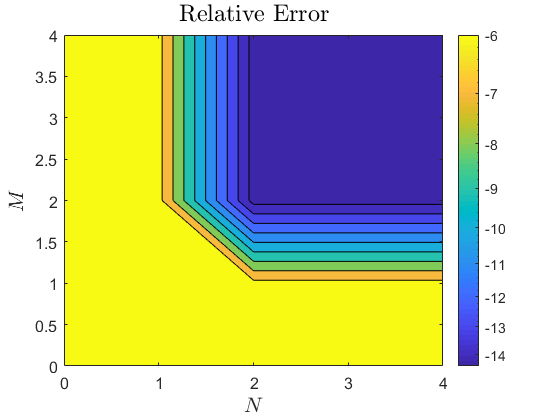
\includegraphics[width=7.6cm]{sections/2_upper_field/Error_Pade_Zeta_U_Good_Profile_N_M_4.png} }}
    \subfloat[Error $\nu^u_r$ (Padé) ]
    {{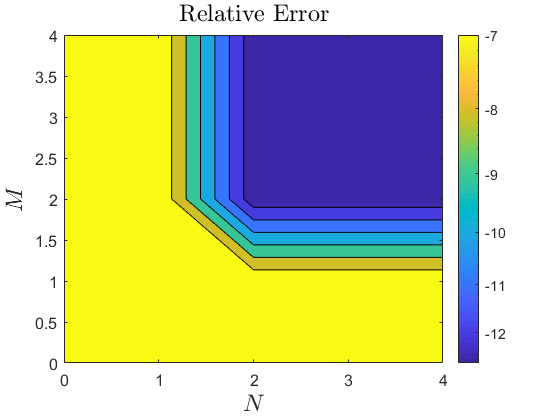
\includegraphics[width=7.6cm]{sections/2_upper_field/Error_Pade_Nu_U_Good_Profile_N_M_4.png} }}
%\includegraphics[width=0.5\textwidth]{conv_N}
\vspace{3mm}
\caption{Plot of Relative Error for $\zeta^u_r$ and $\nu^u_r$ with fixed $\varepsilon = 10^{-6}$ and $\delta = 10^{-8}$. Our HOPS/AWE algorithm used Padé summation and expanded through $0\leq N,M \leq 4$ Padé orders. Physical parameters are reported in the analytic profile above.}
%\label{Fig:N}
\end{figure}




\vspace{-42mm}
\begin{figure}[H]
\centering
    \subfloat[Error ${\zeta^u_r}$ (Padé)]
    {{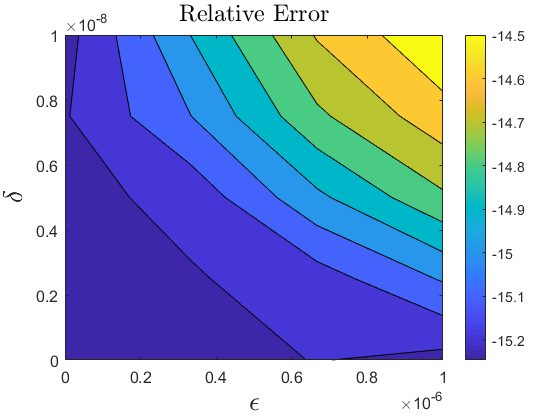
\includegraphics[width=7.6cm]{sections/2_upper_field/Error_Pade_Zeta_U_Good_Profile_Eps_1e-6_Delta_1e-8.png} }}
    \subfloat[Error $\nu^u_r$ (Padé) ]
    {{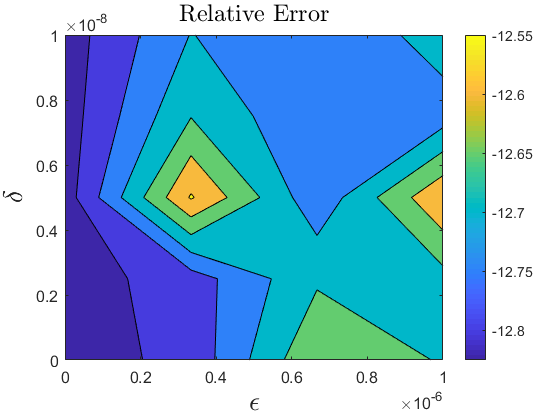
\includegraphics[width=7.6cm]{sections/2_upper_field/Error_Pade_Nu_U_Good_Profile_Eps_1e-6_Delta_1e-8.png} }}
%\includegraphics[width=0.5\textwidth]{conv_N}
\vspace{3mm}
\caption{Plot of Relative Error for $\zeta^u_r$ and $\nu^u_r$ with $N=M=4$ fixed. Our HOPS/AWE algorithm used Padé summation to expand through $0 \leq \varepsilon \leq 10^{-6}$ and $0 \leq \delta \leq 10^{-8}$. Physical parameters are reported in the analytic profile above.}
%\label{Fig:N}
\end{figure}
\vspace{-18mm}
In light of this, we ask the natural question - what is the maximum size of the grating deformation, $\varepsilon$, and frequency perturbation, $\delta$, necessary to achieve spectral accuracy? To investigate we considered a significantly larger perturbation in both $\varepsilon$ and $\delta$ and simulated the same profile with the following parameters
$$f(x)=e^{\cos(x)},\quad \alpha = 0, \quad \varepsilon = 0.02, \quad \delta = 0.001, \quad d=2\pi,\quad r=2,$$
$$A_r=-3,\quad \gamma^u = 1.21, \quad N_x = 32,\quad N_z=32, \quad N=M=4.$$
In Table II we report the results of our tests using both Padé and Taylor summation.
\vspace{3mm}
\label{Second Numerical Tests Upper Layer}
\setcounter{table}{1}
\begin{longtable}[c]{llllll} \toprule
    {$N$} & {$M$} & {Error ${\zeta^w_r}$ (Taylor)} & {Error $\zeta^w_r$ (Padé)} & {Error $\nu^w_r$ (Taylor)} & {Error $\nu^w_r$ (Padé)}  \\ \midrule
0 & 2 & 0.0393875   & 0.0393875   & 0.0151348   & 0.0151348   \\
0 & 4 & 0.0393875   & 0.0393875   & 0.0151348   & 0.0151348   \\
1 & 2 & 0.0393875   & 0.0393875   & 0.0151348   & 0.0151348   \\
1 & 4 & 0.0393875   & 0.0393875   & 0.0151348   & 0.0151348   \\
2 & 2 & 0.00110548  & 2.06154e-05 & 0.000398635 & 1.88162e-05 \\
2 & 4 & 0.00110548  & 2.06154e-05 & 0.000398635 & 1.88162e-05 \\
3 & 2 & 0.00110548  & 2.06154e-05 & 0.000398635 & 1.88162e-05 \\
3 & 4 & 0.00110548  & 2.06154e-05 & 0.000398635 & 1.88162e-05 \\
4 & 2 & 0.00110548  & 2.06154e-05 & 0.000398635 & 1.88162e-05 \\
4 & 4 & 3.23201e-05 & 8.02125e-06 & 1.26113e-05 & 5.0552e-06 \\ \bottomrule
\\
\caption{Relative Error, Error ${\zeta^u_r}$ and Error $\nu^u_r$, versus perturbation orders $N$ and $M$, for the TFE approximations to the Dirichlet data, $\zeta^u_r$ $(2.57\text{a})$, and the Neumann data, $\nu^u_r$ $(2.57\text{b})$, where we used both Taylor Series and Padé approximants. Parameter choices are specified above and both  $\Eps$ and $\delta$ are large.}
\end{longtable}
\vspace{-1mm}
At first, these results are slightly alarming. Continuing in the same manner as the analytic profile, we provide two more figures for the same test parameters. In Figure $6$, we keep $\varepsilon = 0.02$ and $\delta = 0.001$ fixed while we plot the Relative Error for $\zeta^u_r$ and $\nu^u_r$ as we expand through $0\leq N,M \leq 4$ Padé orders. In Figure $7$, we keep $N=M=4$ fixed and plot the Relative Error for $\zeta^u_r$ and $\nu^u_r$ as we expand through $0\leq \varepsilon \leq 0.02$ and $0 \leq \delta \leq 0.001$.

\vspace{-18mm}
\begin{figure}[H]
\centering
    \subfloat[Error ${\zeta^u_r}$ (Padé)]
    {{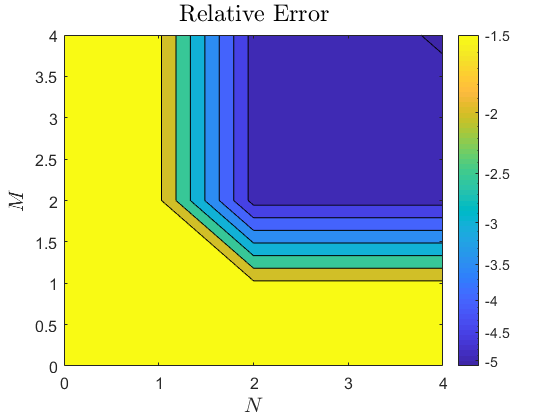
\includegraphics[width=7.6cm]{sections/2_upper_field/Error_Pade_Zeta_U_Bad_Profile_N_M_4.png} }}
    \subfloat[Error $\nu^u_r$ (Padé) ]
    {{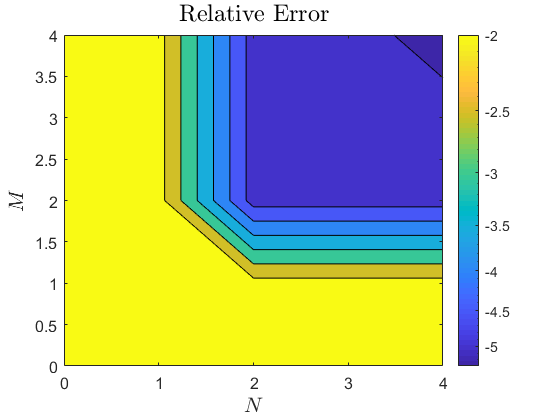
\includegraphics[width=7.6cm]{sections/2_upper_field/Error_Pade_Nu_U_Bad_Profile_N_M_4.png} }}
%\includegraphics[width=0.5\textwidth]{conv_N}
\vspace{3mm}
\caption{Plot of Relative Error for $\zeta^u_r$ and $\nu^u_r$ with fixed $\varepsilon = 0.02$ and $\delta = 0.001$. Our HOPS/AWE algorithm used Padé summation and expanded through $0 \leq N,M \leq 4$ Padé orders. Physical parameters are reported above where both $\Eps$ and $\delta$ are large.}
%\label{Fig:N}
\end{figure}

\vspace{-40mm}
\begin{figure}[H]
\centering
    \subfloat[Error ${\zeta^u_r}$ (Padé)]
    {{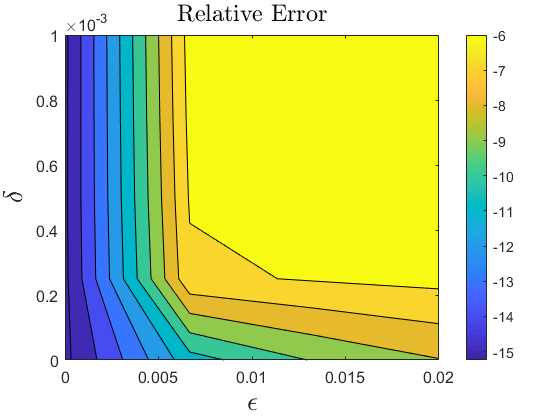
\includegraphics[width=7.6cm]{sections/2_upper_field/Error_Pade_Zeta_U_Bad_Profile_Eps_0.02_Delta_0.001.png} }}
    \subfloat[Error $\nu^u_r$ (Padé) ]
    {{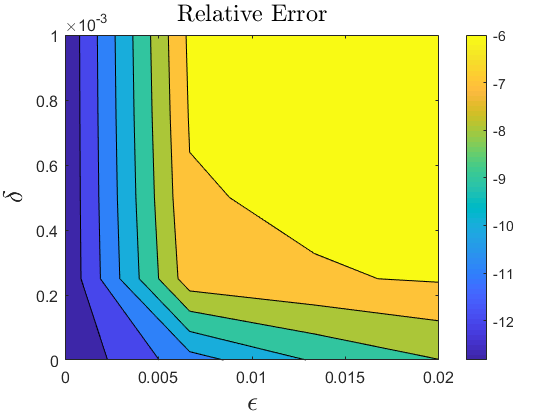
\includegraphics[width=7.6cm]{sections/2_upper_field/Error_Pade_Nu_U_Bad_Profile_Eps_0.02_Delta_0.001.png} }}
%\includegraphics[width=0.5\textwidth]{conv_N}
\vspace{3mm}
\caption{Plot of Relative Error for $\zeta^u_r$ and $\nu^u_r$ with $N=M=4$ fixed. Our HOPS/AWE algorithm used Padé summation to expand through $0 \leq \varepsilon \leq 0.02$ and $0 \leq \delta \leq 0.001$. Physical parameters are reported above where both $\Eps$ and $\delta$ are large.}
%\label{Fig:N}
\end{figure}
\vspace{-19mm}
\begin{flushleft}
We then simulated the same profile with
\end{flushleft}
$$f(x)=e^{\cos(x)},\quad \alpha = 0, \quad \varepsilon = 0.02, \quad \delta = 10^{-6}, \quad d=2\pi,\quad r=2,$$
$$A_r=-3,\quad \gamma^u = 1.21, \quad N_x = 32,\quad N_z=32, \quad N=M=8,$$
where we now expand through $0\leq N,M \leq 8$ Padé orders and have a smaller frequency perturbation. In Figure $8$, we keep $\varepsilon = 0.02$ and $\delta = 10^{-6}$ fixed while we plot the Relative Error for $\zeta^u_r$ and $\nu^u_r$ as we expand through $0 \leq N,M \leq 8$ Padé orders. In Figure $9$, we keep $N=M=8$ fixed and plot the Relative Error for $\zeta^u_r$ and $\nu^u_r$ as we expand through $0\leq \varepsilon \leq 0.02$ and $0 \leq \delta \leq 10^{-6}$.

\vspace{-20mm}
\begin{figure}[H]
\centering
    \subfloat[Error ${\zeta^u_r}$ (Padé)]
    {{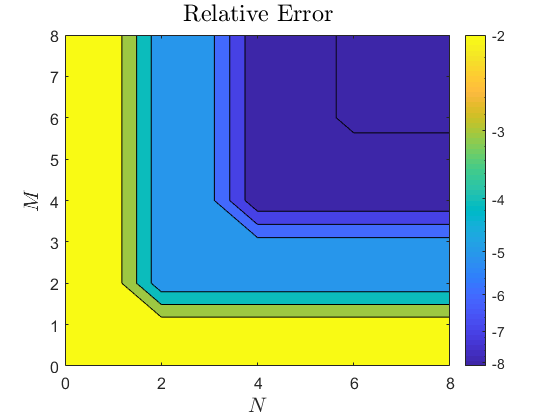
\includegraphics[width=7.6cm]{sections/2_upper_field/Error_Pade_Zeta_U_Intermediate_Profile_N_M_8.png} }}
    \subfloat[Error $\nu^u_r$ (Padé) ]
    {{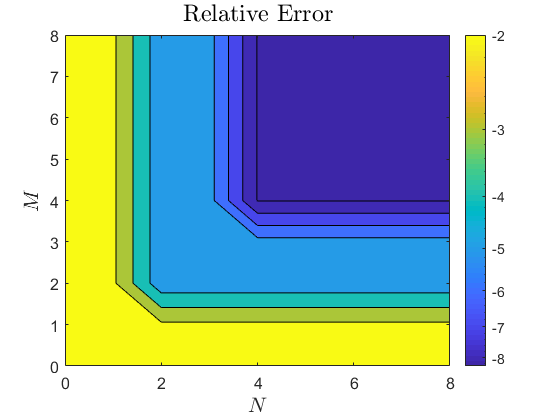
\includegraphics[width=7.6cm]{sections/2_upper_field/Error_Pade_Nu_U_Intermediate_Profile_N_M_8.png} }}
%\includegraphics[width=0.5\textwidth]{conv_N}
\vspace{2mm}
\caption{Plot of Relative Error for $\zeta^u_r$ and $\nu^u_r$ with fixed $\varepsilon = 0.02$ and $\delta = 10^{-6}$. Our HOPS/AWE algorithm used Padé summation to expand through $0 \leq N,M \leq 8$ Padé orders. Physical parameters are reported above where $\Eps$ is large and $\delta$ is small.}
%\label{Fig:N}
\end{figure}

\vspace{-43mm}
\begin{figure}[H]
\centering
    \subfloat[Error ${\zeta^u_r}$ (Padé)]
    {{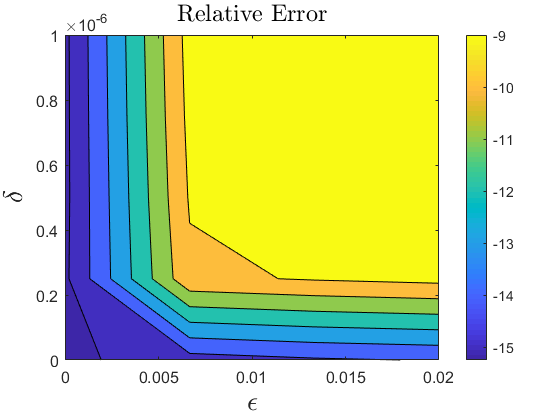
\includegraphics[width=7.6cm]{sections/2_upper_field/Error_Pade_Zeta_U_Intermediate_Profile_Eps_0.02_Delta_1e-6.png} }}
    \subfloat[Error $\nu^u_r$ (Padé) ]
    {{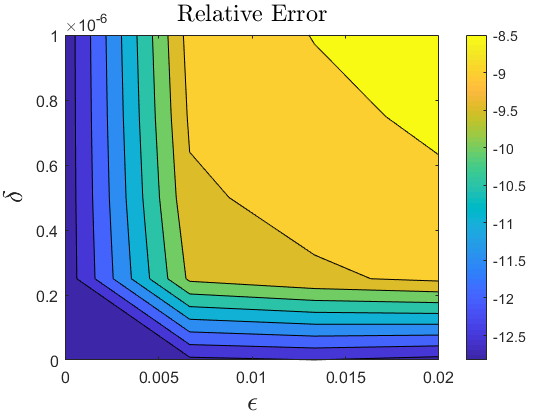
\includegraphics[width=7.6cm]{sections/2_upper_field/Error_Pade_Nu_U_Intermediate_Profile_Eps_0.02_Delta_1e-6.png} }}
%\includegraphics[width=0.5\textwidth]{conv_N}
\vspace{2mm}
\caption{Plot of Relative Error for $\zeta^u_r$ and $\nu^u_r$ with $N=M=8$ fixed. Our HOPS/AWE algorithm used Padé summation to expand through $0 \leq \varepsilon \leq 0.02$ and $0 \leq \delta \leq 10^{-6}$. Physical parameters are reported above where $\Eps$ is large and $\delta$ is small.}
%\label{Fig:N}
\end{figure}
\vspace{-17mm}
Further testing shows that our HOPS/AWE algorithm is better suited towards larger perturbations of $\varepsilon$, which deforms the surface $z=g(x)$, in comparison to large deformations of $\delta$, the frequency. Several factors may be contributing to this effect, including the method by which the DNO, $G$, recovers surface data from the transformed field. As a result, a more detailed analysis will be performed in Chapter $7$. In Appendix A, we provide several code samples which highlight some of our Matlab work. The first subroutine discusses the strategy used to calculate the transformed field, $u=u(x,y;\varepsilon,\delta)$, while the second subroutine explains how we calculate interfacial data by the upper layer DNO, and the third subroutine clarifies how we invert the operator $\bA_{0,0}$. We are now ready to analyze the lower field.

